\documentclass[./../main.tex]{subfiles}
\graphicspath{{img/}}

\begin{document}
    % \problempts{15}

    \section{}

    Para el circuito de la figura siguiente, calcule las probabilidades de los estados \(\ket{0}\) y \(\ket{1}\) en el primer qubit, en términos de \(\abs{\braket{\phi}{\psi}}^{2}\).

    \begin{figure}[htb]
        \centering
        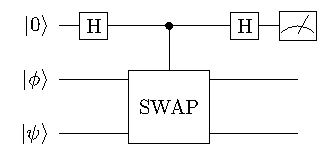
\includegraphics[scale=1.3]{second-circuit.pdf}
        \label{fig:second-circuit}
    \end{figure}

    \startsolution

    Para calcular las probabilidades de los estados \(\ket{0}\) y \(\ket{1}\), primero determinemos el estado final del sistema. Calculamos \(\ket{\Psi_{1}}\),

    \begin{align*}
        \ket{\Psi_{1}} &= (\tensprod{\op{H}}{\op{H}}[\op{I}][nopar])(\tensprod{\ket{0}}{\ket{\phi}}[\ket{\psi}][nopar]),\\
        &= \tensprod{\op{H}\ket{0}}{\ket{\phi}}[\ket{\psi}][nopar],\\
        &= \tensprod{\bigl(\tfrac{1}{\sqrt{2}}\bigl(\ket{0} + \ket{1}\bigr)\bigr)}{\ket{\phi}}[\ket{\psi}][nopar],\\
        \Aboxedsec{\ket{\Psi_{1}} &= \tfrac{1}{\sqrt{2}}\ket{0}\ket{\phi}\ket{\psi} + \tfrac{1}{\sqrt{2}}\ket{1}\ket{\phi}\ket{\psi}}.
    \end{align*}

    La siguiente compuerta a aplicar es la compuerta Fredkin o \(\mathrm{CSWAP}\) que opera sobre tres qubits. Si el qubit control es \(\ket{0}\) los qubits restantes permanecen igual, si es \(\ket{1}\) los qubits restantes invierten su orden. Así,

    \begin{align*}
        \ket{\Psi_{2}} &= \mathrm{CSWAP}\ket{\Psi_{1}},\\
        &= \tensprod{\mathrm{CSWAP}}{\bigl(\tfrac{1}{\sqrt{2}}\ket{0}\ket{\phi}\ket{\psi} + \tfrac{1}{\sqrt{2}}\ket{1}\ket{\phi}\ket{\psi}\bigr)},\\
        &= \tfrac{1}{\sqrt{2}}\Bigl(\mathrm{CSWAP}\ket{0\phi\psi} + \mathrm{CSWAP}\ket{1\phi\psi}\Bigr),\\
        \Aboxedsec{\ket{\Psi_{2}} &= \tfrac{1}{\sqrt{2}}\Bigl(\ket{0\phi\psi} + \ket{1\psi\phi}\Bigr).}
    \end{align*}

    \pagebreak
    Finalmente, aplicamos la compuerta de Hadamard al primer qubit,

    \begin{align*}
        \ket{\Psi_{3}} &= (\tensprod{\op{H}}{\op{I}}[\op{I}][nopar])\tfrac{1}{\sqrt{2}}\Bigl(\ket{0}\ket{\phi\psi} + \ket{1}\ket{\psi\phi}\Bigr),\\
        &= \tfrac{1}{\sqrt{2}}\bigl[\op{H}\ket{0}\ket{\phi\psi} + \op{H}\ket{1}\ket{\psi\phi}\bigr],\\
        &= \tfrac{1}{\sqrt{2}}\Bigl[\tfrac{1}{\sqrt{2}}\bigl(\ket{0} + \ket{1}\bigr)\ket{\phi\psi} + \tfrac{1}{\sqrt{2}}\bigl(\ket{0} - \ket{1}\bigr)\ket{\psi\phi}\Bigr],\\
        \Aboxedsec{\ket{\Psi_{3}} &= \tfrac{1}{2}\ket{0\phi\psi} + \tfrac{1}{2}\ket{1\phi\psi} + \tfrac{1}{2}\ket{0\psi\phi} - \tfrac{1}{2}\ket{1\psi\phi}.}
    \end{align*}

    Para determinar las probabilidades de los estados \(\ket{0}\) y \(\ket{1}\), usamos la expresión

    \begin{equation*}
        p(a_{i}) = \matrixel{\psi}{\hc{M}{a_{i}}\op{M}{a_{i}}}{\psi},
    \end{equation*}

    donde \(\hc{M}{a_{i}} = \proj{i}\) es el operador de proyección asociado al posible resultado \(\{a_{i}\}\) y \(\hc{M}{a_{i}}\) es el resultado de aplicar el operador \(\dagger\) a \(\op{M}{a_{i}}\).

    Entonces, la probabilidad del estado \(\ket{0}\) es

    \begin{align*}
        p(0) &= \dfrac{1}{2}\matrixel{\Psi_{3}}{\proj{0}}{\Psi_{3}},\\
        &= \dfrac{1}{2}\Bigl[\bra{0}(\bra{\phi\psi} + \bra{\psi\phi}) + \bra{1}(\bra{\phi\psi} - \bra{\psi\phi})\Bigr]\Bigl[(\proj{0})\dfrac{1}{2}\Bigl(\ket{0}(\ket{\phi\psi} + \ket{\psi\phi}) + \ket{1}(\ket{\phi\psi} - \ket{\psi\phi})\Bigr)\Bigr],\\
        &= \dfrac{1}{2}\Bigl[\bra{0}(\bra{\phi\psi} + \bra{\psi\phi}) + \bra{1}(\bra{\phi\psi} - \bra{\psi\phi})\Bigr]\Bigl[\dfrac{1}{2}\braket{0}{0}\ket{0}(\ket{\phi\psi} + \ket{\psi\phi}) + \dfrac{1}{2}\braket{0}{1}\ket{0}(\ket{\phi\psi} - \ket{\psi\phi})\Bigr],\\
        &= \dfrac{1}{4}\braket{0}{0}(\bra{\phi\psi} + \bra{\psi\phi})(\ket{\phi\psi} + \ket{\psi\phi}) + \dfrac{1}{4}\braket{1}{0}(\bra{\phi\psi} - \bra{\psi\phi})(\ket{\phi\psi} + \ket{\psi\phi}),\\
        &= \dfrac{1}{4}(\bra{\phi\psi} + \bra{\psi\phi})(\ket{\phi\psi} + \ket{\psi\phi}),\\
        &= \dfrac{1}{4}\Bigl[\braket{\phi}{\phi}\braket{\psi}{\psi} + \braket{\phi}{\psi}\braket{\psi}{\phi} + \braket{\psi}{\phi}\braket{\phi}{\psi} + \braket{\psi}{\psi}\braket{\phi}{\phi}\Bigr],\\
        &= \dfrac{1}{4}\Bigl[1 + \abs{\braket{\phi}{\psi}}^{2} + \abs{\braket{\phi}{\psi}}^{2} + 1\Bigr],\\
        &= \dfrac{1}{4}\Bigl[2 + 2\abs{\braket{\phi}{\psi}}^{2}\Bigr],\\
        \Aboxedmain{p(0) &= \dfrac{1}{2}\Bigl[1 + \abs{\braket{\phi}{\psi}}^{2}\Bigr].}
    \end{align*}

    \pagebreak
    De forma análoga, la probabilidad del estado \(\ket{1}\) es

    \begin{align*}
        p(1) &= \dfrac{1}{2}\matrixel{\Psi_{3}}{\proj{1}}{\Psi_{3}},\\
        &= \dfrac{1}{2}\Bigl[\bra{0}(\bra{\phi\psi} + \bra{\psi\phi}) + \bra{1}(\bra{\phi\psi} - \bra{\psi\phi})\Bigr]\Bigl[\tfrac{1}{2}\braket{1}{0}\ket{1}(\ket{\phi\psi} + \ket{\psi\phi}) + \tfrac{1}{2}\braket{1}{1}\ket{1}(\ket{\phi\psi} - \ket{\psi\phi})\Bigr],\\
        &= \dfrac{1}{4}\braket{0}{0}(\bra{\phi\psi} + \bra{\psi\phi})(\ket{\phi\psi} - \ket{\psi\phi}) + \dfrac{1}{4}\braket{1}{1}(\bra{\phi\psi} - \bra{\psi\phi})(\ket{\phi\psi} - \ket{\psi\phi}),\\
        &= \dfrac{1}{4}(\bra{\phi\psi} - \bra{\psi\phi})(\ket{\phi\psi} - \ket{\psi\phi}),\\
        &= \dfrac{1}{4}\Bigl[\braket{\phi}{\phi}\braket{\psi}{\psi} - \braket{\phi}{\psi}\braket{\psi}{\phi} - \braket{\psi}{\phi}\braket{\phi}{\psi} + \braket{\psi}{\psi}\braket{\phi}{\phi}\Bigr],\\
        &= \dfrac{1}{4}\Bigl[2 - 2\abs{\braket{\phi}{\psi}}^{2}\Bigr],\\
        \Aboxedmain{p(1) &= \dfrac{1}{2}\Bigl[1 - \abs{\braket{\phi}{\psi}}^{2}\Bigr].}
    \end{align*}
\end{document}